% gc-11-OptimizationNewton.tex

\documentclass[xcolor=dvipsnames]{beamer}

\usepackage{cancel}
\renewcommand{\CancelColor}{\color{red}}
\usepackage{graphicx}
\usepackage{wrapfig}
\usepackage{colortbl}
\usepackage{alltt}
\definecolor{myblue}{rgb}{0.8,0.85,1}

\mode<presentation>
{
  \usetheme{Warsaw}
  \setbeamercovered{transparent}
}
% \usecolortheme[named=OliveGreen]{structure}
\setbeamertemplate{navigation symbols}{} 
\setbeamertemplate{blocks}[rounded][shadow=true] 

\newcounter{expls}
\setcounter{expls}{0}
\newcommand{\beispiel}[1]{\refstepcounter{expls}\textbf{Example \arabic{expls}: #1.}}

\newcounter{exercise}
\setcounter{exercise}{0}
\newcommand{\ubung}[0]{\refstepcounter{exercise}\textbf{Exercise \arabic{exercise}: }}

\newif\ifBCITCourse
\BCITCoursetrue
% \BCITCoursefalse
\newif\ifWhichCourse
\WhichCoursetrue
\WhichCoursefalse
\ifBCITCourse
\ifWhichCourse
\newcommand{\CourseName}{Statistics for Food Technology}
\newcommand{\CourseNumber}{MATH 2441}
\newcommand{\CourseInst}{BCIT}
\else
\newcommand{\CourseName}{Calculus for Geomatics}
\newcommand{\CourseNumber}{MATH 2511}
\newcommand{\CourseInst}{BCIT}
\fi
\else
\newcommand{\CourseName}{Philosophy and Literature}
\newcommand{\CourseNumber}{PHIL 375}
\newcommand{\CourseInst}{UBC}
\fi

\title{Newton's Method, Optimization, L'H{\^o}pital's Rule}
\subtitle{{\CourseNumber}, BCIT}

\author{\CourseName}

\date{March 1, 2017}

% \begin{figure}[h]
% 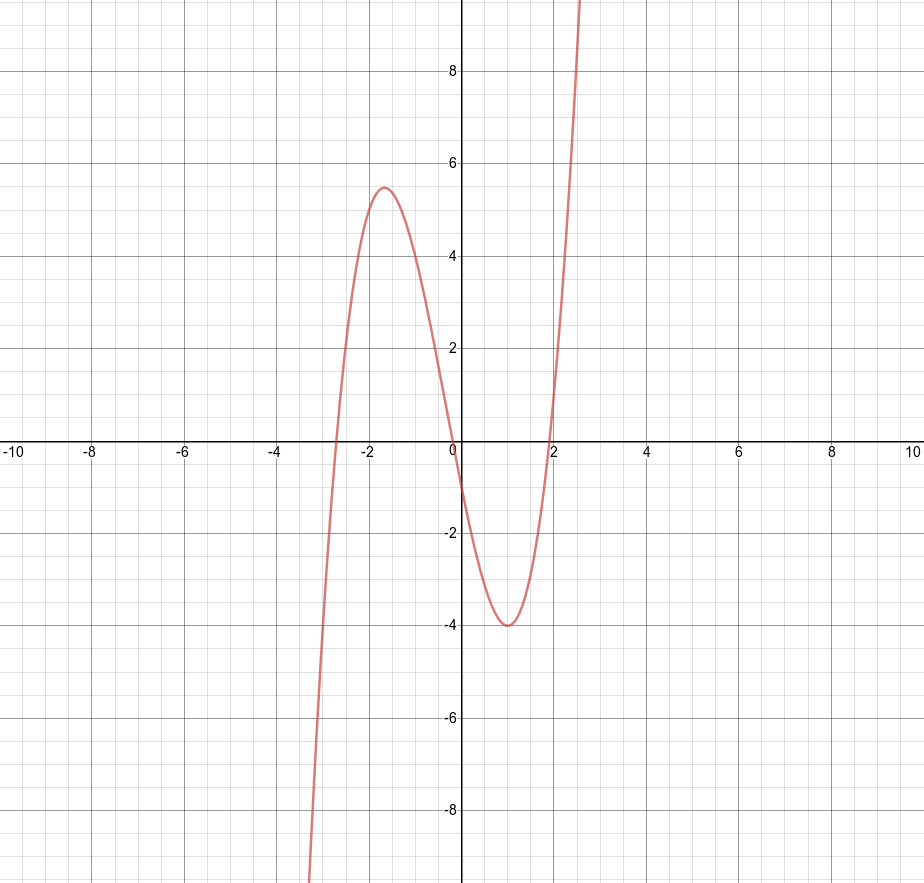
\includegraphics[scale=.3]{./diagrams/extrema1.png}
% \end{figure}

\begin{document}

\begin{frame}
  \titlepage
\end{frame}

%%%%%%%%%%%%%%%%%%%%%%%%%%%%%%%%%%%%%%%%%%%%%%%%%%%%%%%%%%%%%%%%%%
% I created a video for this. See https://youtu.be/a28M5f0Dk_c or find NewtonsMethod.tar.gz.
%%%%%%%%%%%%%%%%%%%%%%%%%%%%%%%%%%%%%%%%%%%%%%%%%%%%%%%%%%%%%%%%%%

\begin{frame}
  \frametitle{Newton's Method}
What are the $x$-intercepts of the following function?
\begin{equation}
  \label{eq:ietaicie}
f(x)=2x^{3}+5x^{2}-11x+3\notag
\end{equation}
% \begin{equation}
%   \label{eq:quohgaiy}
%   \mbox{The algebraic solution is approximately }1.149496\notag
% \end{equation}
We have not learned how to find $x$-intercepts for polynomials with
degrees higher than 2. There are different methods. One method is
called \alert{Newton's Method} and approximates the $x$-intercept. I
have created an instructional video for Newton's Method which you can
watch here:
\begin{alltt}
https://youtu.be/a28M5f0Dk\_c
\end{alltt}
\end{frame}

\begin{frame}
  \frametitle{Newton's Method}
For Newton's Method, find a plausible $x$-value $x_{1}$ (near enough
to the $x$-intercept that you are trying to find) and approximate the
$x$-intercept using the following iterative procedure:
\begin{equation}
  \label{eq:heimioje}
  x_{n+1}=x_{n}-\frac{f(x_{n})}{f'(x_{n})}
\end{equation}
\end{frame}

\begin{frame}
  \frametitle{Exercise}
{\ubung} Approximate $\sqrt{7}$ to ten decimal places using Newton's
  method and the function $h(x)=x^{2}-7$. 
\end{frame}

\begin{frame}
  \frametitle{Exercise}
{\ubung} Approximate the $x$-intercept of $f(x)=x^{3}+5x-3$ using
  Newton's method. % 0.5641
\end{frame}

\begin{frame}
  \frametitle{Exercise}
{\ubung} Factor $g(t)=24t^{3}-2t^{2}-9t+2$. Remember that if $x_{1},x_{2},x_{3}$ 
  are $x$-intercepts of the polynomial $ax^{3}+bx^{2}+cx+d$, then
  \begin{equation}
    \label{eq:ahsuagha}
    ax^{3}+bx^{2}+cx+d=a(x-x_{1})(x-x_{2})(x-x_{3})
  \end{equation}
% solution: (x-1/2)(x+2/3)(x-1/4)
\end{frame}

\begin{frame}
  \frametitle{Exercise}
{\ubung} Find the $x$-intercepts for the following function:
\begin{equation}
  \label{eq:yiceepuo}
  f(x)=x^{3}+4x^{2}+x-6
\end{equation}
\end{frame}

\begin{frame}
  \frametitle{Exercise}
{\ubung} Solve the equation
\begin{equation}
  \label{eq:puxeepha}
  \cos{}x=x
\end{equation}
using Newton's Method.
\end{frame}

\begin{frame}
  \frametitle{Exercise}
{\ubung} Analyze the following function:
\begin{equation}
  \label{eq:aehoilao}
  f(x)=\frac{2x^{2}+2}{x-3}
\end{equation}
\end{frame}

\begin{frame}
  \frametitle{Exercise}
{\ubung} Solve the following equations using Newton's Method. Use a
graphing calculator to get you started.
\begin{equation}
  \label{eq:xeigheuy}
  x^{6}-x^{5}-6x^{4}-x^{2}+x+10=0
\end{equation}
\begin{equation}
  \label{eq:ohtharoh}
  x^{2}(4-x^{2})=\frac{4}{x^{2}+1}
\end{equation}
\begin{equation}
  \label{eq:iejuangi}
  x^{2}\sqrt{2-x-x^{2}}=1
\end{equation}
\begin{equation}
  \label{eq:oungiegu}
  4e^{-x^{2}}\sin{}x=x^{2}-x+1
\end{equation}
\begin{equation}
  \label{eq:ohpaejae}
  3\sin(x^{2})=2x
\end{equation}
\end{frame}

\begin{frame}
  \frametitle{Exercise}
{\ubung} Find the absolute minimum value of the following function
correct to four decimal places.
\begin{equation}
  \label{eq:veiyeini}
  f(x)=x^{6}-x^{4}+3x^{2}-2x
\end{equation}
\end{frame}

\begin{frame}
  \frametitle{Exercise}
{\ubung} Of the infinitely many lines that are tangent to the curve
\begin{equation}
  \label{eq:ohtooyiv}
  y=-\sin{}x
\end{equation}
and pass through the origin, there is one that has the largest slope.
Use Newton's Method to find the slope of that line.
\end{frame}

\begin{frame}
  \frametitle{Exercise}
{\ubung} Use Newton's Method to find the coordinates of the point on
the parabola
\begin{equation}
  \label{eq:laingiun}
  y=(x-1)^{2}
\end{equation}
that is closest to the origin.
\end{frame}

\begin{frame}
  \frametitle{Optimization}
  The last exercise gives us a nice segue to \alert{optimization}. You
  already have all the tools for optimization. Optimization is often a
  matter of finding the solutions for $f'(x)=0$ and then checking the
  second derivative to make sure the solution is what you were looking
  for. However, finding the function $f(x)$ can sometimes (as in the
  last exercise) be tricky! Here are some exercises.
\end{frame}

\begin{frame}
  \frametitle{Exercise}
  {\ubung} A farmer has 2400ft of fencing and wants to fence off a
  rectangular field that borders a straight river. She needs no fence
  along the river. What are the dimensions of the field that has the
  largest area?
\end{frame}

\begin{frame}
  \frametitle{Exercise}
  {\ubung} A cylindrical can is to be made to hold one litre of oil.
  Find the dimensions that wil minimize the cost of the metal to
  manufacture the can.
\end{frame}

\begin{frame}
  \frametitle{Exercise}
  {\ubung} Find the area of the largest rectangle that can be
  inscribed in a semicircle of radius $r$.
\end{frame}

\begin{frame}
  \frametitle{Exercise}
  {\ubung} A cone with height $h$ and radius $r$ is inscribed in a
  larger cone with height $H$ and radius $R$ so that its vertex is at
  the centre of the base of the larger cone. Find $h$ in terms of the
  dimensions of the larger cone that makes the volume of the smaller
  cone maximal.
\begin{figure}[h]
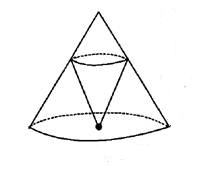
\includegraphics[scale=.75]{./diagrams/coneopt.png}
\end{figure}
\end{frame}

\begin{frame}
  \frametitle{Exercise}
  {\ubung} For a fish swimming at a speed $v$ relative to the water,
  the energy expenditure per unit time is proportional to $v^{3}$. It
  is believed that migrating fish try to minimize the total energy
  required to swim a fixed distance. If the fish are swimming against
  a current $u$ ($u<v$), then the time required to swim a distance $L$
  is $L/(v-u)$ and the total energy $E$ required to swim the distance
  is given by
  \begin{equation}
    \label{eq:aiyeiyoo}
    E(v)=av^{3}\cdot\frac{L}{v-u}
  \end{equation}
  where $a$ is the proportionality constant. Determine the value of
  $v$ that minimizes $E$.
\end{frame}

\begin{frame}
  \frametitle{Exercise}
  {\ubung} How close does the semi-circle $y=\sqrt{16-x^{2}}$ come to
  the point $P=(1,\sqrt{3})$?
\end{frame}

\begin{frame}
  \frametitle{Exercise Solution}
  Note that the semi-circle $y=\sqrt{16-x^{2}}$ is part of a circle
  with a centre of $M=(0,0)$ and radius $r=4$. If $Q=(x,y)$ is the
  point on the semi-circle closest to $P$, then the distance between
  $P$ and $Q$ is
\begin{equation}
  \label{eq:aziobaeg}
  f(x)=\sqrt{(x-1)^{2}+(y-\sqrt{3})^{2}}
\end{equation}
Since $Q$ is on the semi-circle, we can replace $y=\sqrt{16-x^{2}}$ to
get 
\begin{equation}
  \label{eq:shahquua}
  f(x)=\sqrt{(x-1)^{2}+(\sqrt{16-x^{2}}-\sqrt{3})^{2}}
\end{equation}
\end{frame}

\begin{frame}
  \frametitle{Exercise Solution}
  The distance between $P$ and $Q$ is
\begin{equation}
  \label{eq:ohghoote}
  f(x)=\sqrt{(x-1)^{2}+(\sqrt{16-x^{2}}-\sqrt{3})^{2}}=\sqrt{g(x)}
\end{equation}
Call the expression under the square root sign $g(x)$. Then
\begin{equation}
  \label{eq:ouwophai}
  f'(x)=\frac{1}{2}\cdot\left(g(x)\right)^{-\frac{1}{2}}\cdot{}g'(x)
\end{equation}
Of these three factors, only $g'(x)$ can be zero. Setting $f'(x)=0$ is
therefore equivalent to $g'(x)=0$. Note that
\begin{equation}
  \label{eq:poqueebo}
  g'(x)=2(x-1)+2\left(\sqrt{16-x^{2}}-\sqrt{3}\right)\cdot\left(\frac{1}{2}(16-x^{2})^{-\frac{1}{2}}\cdot(-2x)\right)\notag
\end{equation}
\end{frame}

\begin{frame}
  \frametitle{Exercise Solution}
Simplify and expand to
\begin{equation}
  \label{eq:deiquoot}
  \frac{1}{2}g'(x)=(x-1)-x+\frac{\sqrt{3}x}{\sqrt{16-x^{2}}}
\end{equation}
$g'(x)=0$ just when
\begin{equation}
  \label{eq:xoonahju}
  1=\frac{\sqrt{3}x}{\sqrt{16-x^{2}}}
\end{equation}
Square both sides for the polynomial equation
\begin{equation}
  \label{eq:uabaevoo}
4x^{2}-16=0
\end{equation}
and the two solutions $x_{1}=-2$ and $x_{2}=2$. The first solution is
where the distance between $P$ and $Q$ is at a maximum. The second
solution is where the distance is at a minimum. Therefore, the point
$Q=(2,2\sqrt{3})$ is the answer to the question in this exercise.
\end{frame}

\begin{frame}
  \frametitle{L'H{\^o}pital's Rule}
Evaluate the following limits:
\begin{equation}
  \label{eq:ohjishah}
  \lim_{x\rightarrow{}1}\frac{x^{2}-x}{x^{2}-1}
\end{equation}
\begin{equation}
  \label{eq:eighahth}
  \lim_{x\rightarrow{}0}\frac{\sin{}x}{x}\mbox{ (it equals 1 based on geometry)}
\end{equation}
\begin{equation}
  \label{eq:aiwohmae}
  \lim_{x\rightarrow\infty}\frac{x^{2}-1}{2x^{2}+1}
\end{equation}
These limits have in common that they are of \alert{indeterminate
  form} when you plug in the $a$ towards which the $x$ goes. Sometimes
the tricks we have found don't work, for example for
\begin{equation}
  \label{eq:jechuith}
  \lim_{x\rightarrow{}1}\frac{\ln{}x}{x-1}
\end{equation}
or for
\begin{equation}
  \label{eq:ieghaegh}
  \lim_{x\rightarrow{}\infty}\frac{\ln{}x}{x-1}
\end{equation}
\end{frame}

\begin{frame}
  \frametitle{L'H{\^o}pital's Rule}
\begin{figure}[h]
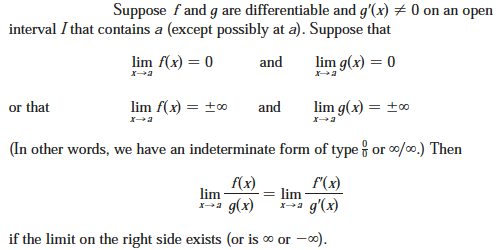
\includegraphics[scale=.6]{./diagrams/lhopital_ed.png}
\end{figure}
\end{frame}

\begin{frame}
  \frametitle{Exercise}
{\ubung} Find
\begin{equation}
  \label{eq:aimooshi}
  \lim_{x\rightarrow{}1}\frac{\ln{}x}{x-1}
\end{equation}
\end{frame}

\begin{frame}
  \frametitle{Exercise}
{\ubung} Find
\begin{equation}
  \label{eq:awaifeif}
  \lim_{x\rightarrow\infty}\frac{e^{x}}{x^{2}}
\end{equation}
\end{frame}

\begin{frame}
  \frametitle{Exercise}
  {\ubung} Find
  \begin{equation}
    \label{eq:ijieyoja}
    \lim_{x\rightarrow\infty}\frac{\ln{}x}{\sqrt[3]{x}}
  \end{equation}
\end{frame}

\begin{frame}
  \frametitle{Exercise}
  {\ubung} Find
  \begin{equation}
    \label{eq:iemohyua}
    \lim_{x\rightarrow{}0}\frac{\tan{}x-x}{x^{3}}
  \end{equation}
% Solution is 1/3
\end{frame}

\begin{frame}
  \frametitle{Exercise}
  {\ubung} Fynd
  \begin{equation}
    \label{eq:eekuyuoc}
    % \lim_{x\rightarrow\pi^{-}}\frac{\sin{}x}{1-\cos{}x}
    \lim_{x\rightarrow\pi}\frac{\pi-\pi\cos{}x+\sin{}x}{1-\cos{}x}
  \end{equation}
\end{frame}

\begin{frame}
  \frametitle{Exercise}
  {\ubung} Find
  \begin{equation}
    \label{eq:zeisahda}
    \lim_{x\rightarrow{}0^{+}}x\ln{}x
  \end{equation}
\end{frame}

\begin{frame}
  \frametitle{Exercise}
  {\ubung} Find
  \begin{equation}
    \label{eq:ahgohgah}
    \lim_{x\rightarrow\frac{\pi}{2}^{-}}(\sec{}x-\tan{}x)
  \end{equation}
\end{frame}

\begin{frame}
  \frametitle{Exercise}
  {\ubung} Find
  \begin{equation}
    \label{eq:xughieta}
    \lim_{x\rightarrow{}0^{+}}(1+\sin{}4x)^{\cot{}x}
  \end{equation}
\end{frame}

\begin{frame}
  \frametitle{Exercise}
  {\ubung} Find
  \begin{equation}
    \label{eq:mahpeilu}
    \lim_{x\rightarrow{}0^{+}}x^{x}
  \end{equation}
\end{frame}

\begin{frame}
  \frametitle{Exercise}
  {\ubung} Find
  \begin{equation}
    \label{eq:eigahrai}
    \lim_{x\rightarrow\infty}(\sqrt{x^{2}+x}-x)
  \end{equation}
\end{frame}

\begin{frame}
  \frametitle{Exercise}
  {\ubung} Find
  \begin{equation}
    \label{eq:vuciecha}
    \lim_{x\rightarrow{}1}\frac{1-x+\ln{}x}{1+\cos\pi{}x}
  \end{equation}
\end{frame}

\begin{frame}
  \frametitle{Exercise}
  {\ubung} Find
  \begin{equation}
    \label{eq:taihahri}
    \lim_{x\rightarrow{}0}\frac{e^{x}-e^{-x}-2x}{x-\sin{}x}
  \end{equation}
\end{frame}

\begin{frame}
  \frametitle{Exercise}
  {\ubung} Find
  \begin{equation}
    \label{eq:eemeeyae}
    \lim_{x\rightarrow{}0^{+}}\sin{}x\ln{}x
  \end{equation}
\end{frame}

\begin{frame}
  \frametitle{Exercise}
  {\ubung} Find
  \begin{equation}
    \label{eq:gasuchoh}
    \lim_{x\rightarrow{}1}\left(\frac{x}{x-1}-\frac{1}{\ln{}x}\right)
  \end{equation}
\end{frame}

\begin{frame}
  \frametitle{End of Lesson}
Next Lesson: Fundamental Theorem of Calculus
\end{frame}

\end{document}

